\documentclass[10pt]{extarticle}
\title{}
\author{Avinash Iyer}
\date{}
\usepackage[shortlabels]{enumitem}

%font setup
%
%\usepackage{newpxtext,eulerpx}

%paper setup
\usepackage{geometry}
\geometry{letterpaper, portrait, margin=1in}
\usepackage{fancyhdr}

%symbols
\usepackage{amsmath}
\usepackage{amssymb}
\usepackage{mathtools}
\usepackage{hyperref}
\usepackage{gensymb}
\usepackage{multirow,array}

\usepackage[T1]{fontenc}
\usepackage[utf8]{inputenc}

%chemistry stuff
\usepackage[version=4]{mhchem}
\usepackage{chemfig}

%plotting
\usepackage{pgfplots}
\usepackage{tikz}
\tikzset{middleweight/.style={pos = 0.5, fill=white}}
\tikzset{weight/.style={pos = 0.5, fill = white}}
\tikzset{lateweight/.style={pos = 0.75, fill = white}}
\tikzset{earlyweight/.style={pos = 0.25, fill=white}}

%\usepackage{natbib}

%graphics stuff
\usepackage{graphicx}
\graphicspath{ {./images/} }

%code stuff
%when using minted, make sure to add the -shell-escape flag
%you can use lstlisting if you don't want to use minted
%\usepackage{minted}
%\usemintedstyle{pastie}
%\newminted[javacode]{java}{frame=lines,framesep=2mm,linenos=true,fontsize=\footnotesize,tabsize=3,autogobble,}
%\newminted[cppcode]{cpp}{frame=lines,framesep=2mm,linenos=true,fontsize=\footnotesize,tabsize=3,autogobble,}

%\usepackage{listings}
%\usepackage{color}
%\definecolor{dkgreen}{rgb}{0,0.6,0}
%\definecolor{gray}{rgb}{0.5,0.5,0.5}
%\definecolor{mauve}{rgb}{0.58,0,0.82}
%
%\lstset{frame=tb,
%	language=Java,
%	aboveskip=3mm,
%	belowskip=3mm,
%	showstringspaces=false,
%	columns=flexible,
%	basicstyle={\small\ttfamily},
%	numbers=none,
%	numberstyle=\tiny\color{gray},
%	keywordstyle=\color{blue},
%	commentstyle=\color{dkgreen},
%	stringstyle=\color{mauve},
%	breaklines=true,
%	breakatwhitespace=true,
%	tabsize=3
%}
% text + color boxes
\usepackage[most]{tcolorbox}
\tcbuselibrary{breakable}
\newtcolorbox{problem}[1]{colback = white, title = {#1}, breakable}
\newtcolorbox{solution}{colback = white, colframe = black!75!white, title = Solution, breakable}
%including PDFs
%\usepackage{pdfpages}
\setlength{\parindent}{0pt}

\pagestyle{fancy}
\fancyhf{}
\rhead{Avinash Iyer}
\lhead{Econ 308: Problem Set 2}
\newcommand{\card}{\text{card}}
\newcommand{\ran}{\text{ran}}
\newcommand{\N}{\mathbb{N}}
\newcommand{\Q}{\mathbb{Q}}
\newcommand{\Z}{\mathbb{Z}}
\newcommand{\R}{\mathbb{R}}
\begin{document}
  \begin{problem}{Optimal Pigouvian Taxation}
    A coal-fired power plant releases air pollution into the atmosphere for every unit of electricity produced. The inverse demand function is $P_d = 20 - 0.5Q$, which represents the marginal benefit where $Q$ is the quantity consumed when consumers pay price $P_d$. The inverse supply curve for coal-fired electricity is $P_s = 5 + Q$, which represents the marginal private cost curve when the power plant produces $Q$ units. The marginal damage from emissions is given by $MD = 3.5Q$, which describes the cost of greenhouse gas emissions and local air pollution when the industry generates $Q$ units of coal-fired electricity.
    \begin{enumerate}[(a)]
      \item Illustrate the market for the coal-fired electricity with a supply/demand graph. Be sure to draw the curves for demand, supply, marginal damage, and social marginal cost.
      \item What is the private market equilibrium?
      \item What is the socially optimal/efficient quantity of coal-fired electricity?
      \item How large is the deadweight loss from this negative production externality?
      \item A corrective tax has the effect of ``internalizing the externality.'' How large should the (constant) per-unit corrective tax be in order to induce the market quantity to be socially optimal/efficient? Draw the firm's supply curve with the new tax on your graph in part (a). What is the consumer price paid and the supplier price received with the optimal corrective tax?
    \end{enumerate}
    \tcblower
    \begin{problem}{(a)}
      \begin{center}
        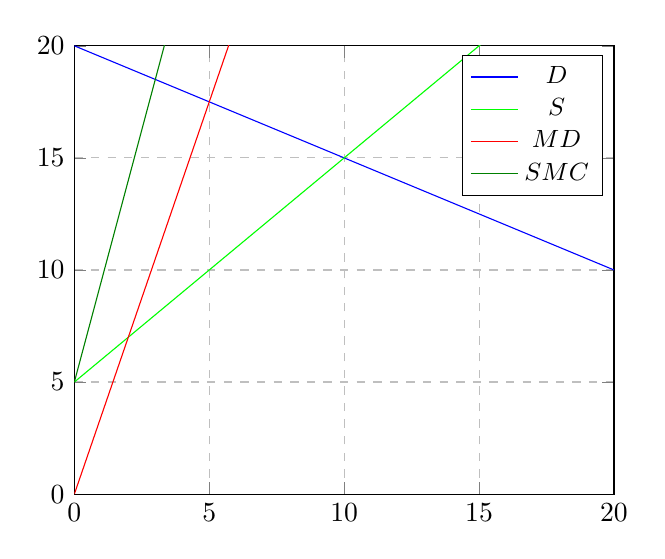
\begin{tikzpicture}
          \begin{axis}[
            xtick={0,5,10,15,20},
            ytick={0,5,10,15,20},
            xmin=0,xmax=20,ymin=0,ymax=20,xmajorgrids=true,ymajorgrids=true,grid style = dashed
            ]
            \addplot[domain = 0:20,color=blue]{20-0.5*x};
            \addlegendentry{\small $D$}
            \addplot[domain = 0:20,color = green]{5+x};
            \addlegendentry{\small $S$};
            \addplot[domain = 0:20,color = red]{3.5*x};
            \addlegendentry{\small $MD$}
            \addplot[domain = 0:20,color = green!50!black]{5 + 4.5*x};
            \addlegendentry{\small $SMC$};
          \end{axis}
        \end{tikzpicture}
      \end{center}
    \end{problem}
    \begin{problem}{(b)}
      \begin{align*}
        20-0.5Q &= 5 + Q\\
        15 &= 1.5Q\\
        Q &= 10\\
        P &= 15
      \end{align*}
    \end{problem}
    \begin{problem}{(c)}
      \begin{align*}
        20-0.5Q &= 5+Q+3.5Q\\
        15 &= 5Q\\
        Q &= 3\\
        P &= 18.5
      \end{align*}
    \end{problem}
    \begin{problem}{(d)}
      \begin{align*}
        DWL &= \frac{1}{2}(\Delta P)(\Delta Q)\\
            &= \frac{1}{2}(3.5)(7)
            &= 12.25
      \end{align*}
    \end{problem}
    \begin{problem}{(e)}
      The firm's per-unit corrective tax should be equal to the marginal damage at the socially optimal quantity, meaning $t = 3.5(3) = 10.5$. The supply curve with the externality internalized is $P_s' = 15.5 + Q$.
      \begin{center}
        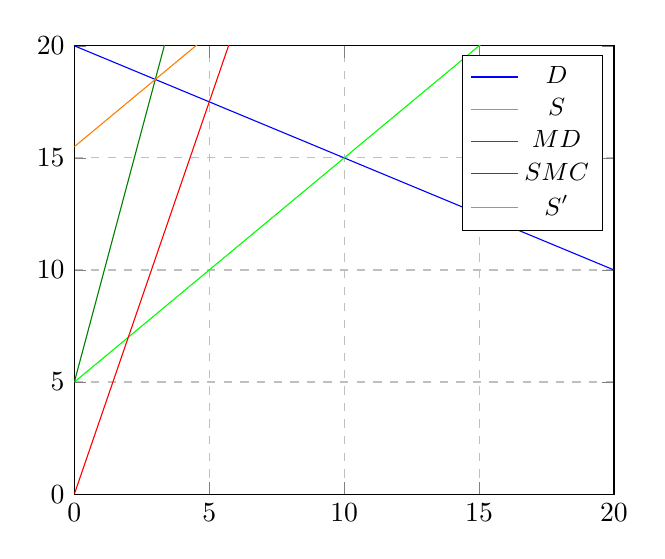
\begin{tikzpicture}
          \begin{axis}[
            xtick={0,5,10,15,20},
            ytick={0,5,10,15,20},
            xmin=0,xmax=20,ymin=0,ymax=20,xmajorgrids=true,ymajorgrids=true,grid style = dashed
            ]
            \addplot[domain = 0:20,color=blue]{20-0.5*x};
            \addlegendentry{\small $D$}
            \addplot[domain = 0:20,color = green]{5+x};
            \addlegendentry{\small $S$};
            \addplot[domain = 0:20,color = red]{3.5*x};
            \addlegendentry{\small $MD$}
            \addplot[domain = 0:20,color = green!50!black]{5 + 4.5*x};
            \addlegendentry{\small $SMC$};
            \addplot[domain = 0:20,color = orange]{15.5+x};
            \addlegendentry{\small $S'$};
          \end{axis}
        \end{tikzpicture}
      \end{center}
    \end{problem}
  \end{problem}
  \begin{problem}{Pollution Standards}
    Another way to reduce pollution is to mandate a maximum quantity of pollution (instead of taxing pollution-creating activities). Chay and Greenstone (2005) study the impact of the standards created by the 1970 Clean Air Act. They explain that:
    \begin{quote}
      Before 1970 the federal government did not play a significant role in the regulation of air pollution; that responsibility was left primarily to state governments. In the absence of federal legislation, few states found it in their interest to impose strict regulations on polluters within their jurisdictions. Concerned with the detrimental health effects of persistently high concentrations of [total suspended particulates] TSPs and other air pollutants, Congress passed the Clean Air Act Amendments of 1970.\\

      The centerpiece of the CAAAs is the establishment of separate federal air quality standards, known as the National Ambient Air Quality Standards, for five pollutants. The stated goal of the amendments is to bring all counties into compliance with the standards by reducing local air pollution concentrations. The legislation requires the EPA to assign annually each county to either nonattainment or attainment status for each of the pollutants, on the basis of whether the relevant standard is exceeded. The federal TSPs standard is violated if either of two thresholds is exceeded: (1) the annual geometric mean concentration exceeds 75 $\mu$g/m$^3$ or (2) the second- highest daily concentration exceeds 260 $\mu$g/m$^3$. (pp. 382-383)\\

      Some counties were already below this ceiling and were therefore in attainment status. But for nonattainment status counties, these new standards required a change in pollution levels. This suggests a diff-in-diff strategy for estimating for the impact of the standards on TSPs. They provide the following visualization of the data:
    \end{quote}
    \begin{center}
      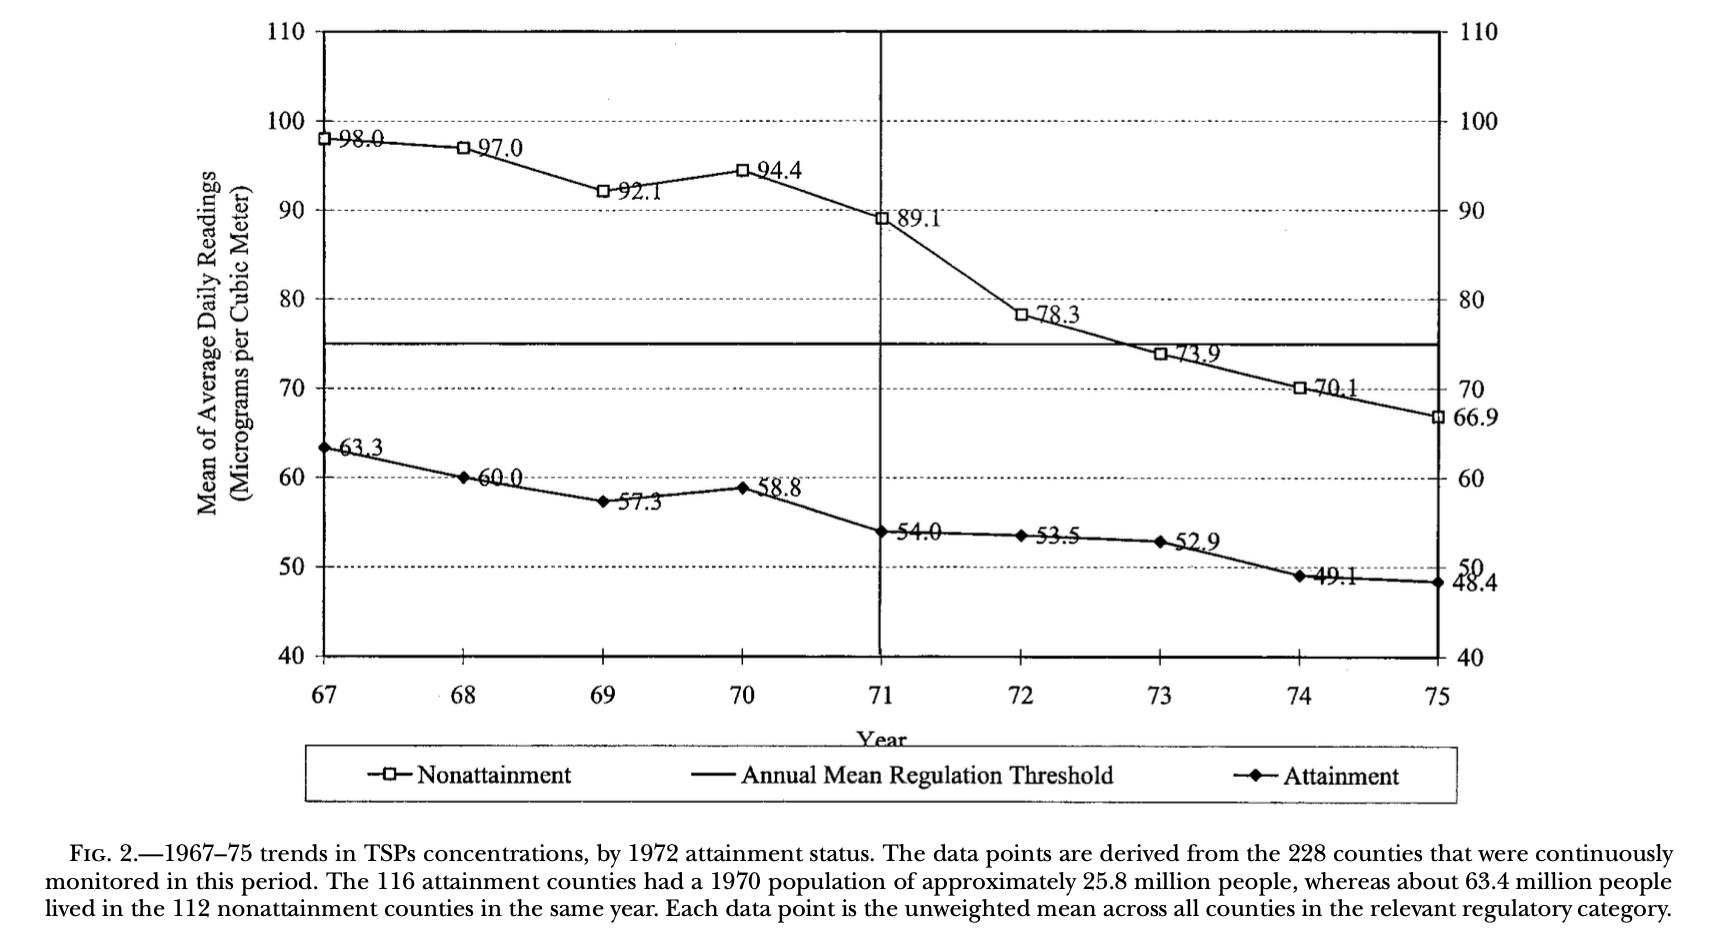
\includegraphics[width=\textwidth]{2_1_q}
    \end{center}
    \begin{enumerate}[(a)]
      \item Which counties are in the ``treatment'' group and which counties are in the ``control'' group?
      \item Let $TSP_{y}^{g}$ indicate the average TSP level in year $y$ for counties in group $G$, where $G = C$ for the control group, and $G = T$ for the treatment group. Compute the average TSP levels for the treatment and control group in the years before and after 1971.
      \item Use the difference-in-differences estimator and the four values you computed in part (b) to derive an estimate of the impact of the new standards on TSP. Interpret this estimate.
      \item What is the key assumption for the DD to identify the causal effect of interest? Does this assumption appear to be satisfied in this case or not?
    \end{enumerate}
    \tcblower
    \begin{problem}{(a)}
      The counties with TSP levels above the threshold were the treatment group, and the counties with TSP levels below the threshold were the control group.
    \end{problem}
    \begin{problem}{(b)}
      \begin{itemize}
        \item $TSP_{T}^{B} = 95.4$
        \item $TSP_{T}^{A} = 72.3$
        \item $TSP_{C}^{B} = 59.9$
        \item $TSP_{C}^{A} = 51.0$
      \end{itemize}
    \end{problem}
    \begin{problem}{(c)}
      The DD estimate is 14.2, implying that the Clean Air Act is responsible for a reduction of 14.2 micrograms per cubic meter in total suspended particulates that did not happen otherwise.
    \end{problem}
    \begin{problem}{(d)}
      The primary assumption for the DD to identify the causal effect is that the treatment group would have acted similar to the control group otherwise --- given that the alternative was the treatment group not being exposed to the Clean Air Act, the treatment counties should have acted similar to the control group, meaning that the assumption should be satisfied.
    \end{problem}
  \end{problem}
  \begin{problem}{Theory and Evidence of Crowd-Out}
    Suppose you have a friend who works in fundraising at the public ratio station in your town. One day she tells you excitedly that the station has just been selected to receive a large grant from the federal government. The marketing department at the station plans to feature details about the grant in an upcoming promotional email, hoping that the news will drive a wave of new donations.
    \begin{enumerate}[(a)]
      \item In general, we would expect that the existence of such a grant would reduce donations via crowd-out, so this email would certainly backfire. Using the theoretical tools of economics, provide two reasons why crowd-out after the receipt of this new government funding would be less than full.
      \item As a budding experimental economist you are interested in the questions about crowd-out that emerged when speaking with your friend about marketing for the local public radio station. You suggest to your friend that this is a perfect opportunity to study crowd-out empirically. You suggest that the station run a small experiment, randomizing the recipients of the email into two groups --- one group receiving an email promoting the new federal grant, and the other receiving an email highlighting the great work the station has done recently, but omitting mention of the grant. How would this improve on Kingma’s 1989 study of public radio? What might be the pitfalls of such an approach?
    \end{enumerate}
    \tcblower
    \begin{problem}{(a)}
      There are other preferences that may result in people choosing to donate even after the grant --- for example, altruism or warm glow preferences may result in people choosing to donate even after the grant, meaning that crowd-out will likely be less than full.
    \end{problem}
    \begin{problem}{(b)}
      This would improve on Kingma's study by randomizing within the same income group (rather than using an aggregation measure that might bias towards less or more crowd-out than actually happens), but it might suffer from other biases like omitted variable bias (such as the idea that people still heard about the grant elsewhere even if they didn't receive it in the email).
    \end{problem}
  \end{problem}
  \begin{problem}{Public Concerts}
    The town of Musicville has two residents: Bach ($B$) and Mozart ($M$). The town currently funds its free outdoor concert series solely from the individual contributions of these residents. Each of the residents has the same utility function over private goods $X$ and concerts $C$, in the form:
    \begin{align*}
      U_B &= 3\ln(X_M) + 2\ln(C)\\
      U_M &= 3\ln(X_M) + 2\ln(C)
    \end{align*}
    The total number of concerts given, $C$, is the sum of the number paid for by each of the two persons: $C = C_B + C_M$. Bach and Mozart combined have incomes of 60, and the price of both the private good and the concert is $1$.
    \begin{enumerate}[(a)]
      \item How many concerts are given if the government does not interfere?
      \item What is the socially optimal number of concerts?
      \item Suppose the government is not happy with the private equilibrium and decides to provide 8 concerts in addition to what Bach and Mozart may choose to provide on their own. It taxes Bach and Mozart equally to pay for the new concerts. What is the new total number of concerts? How does your answer compare to your answers in part (a) and (b)?
      \item Suppose that instead an anonymous benefactor pays for 8 concerts. What is the new total number of concerts? Is this the same level of provision as (c)? Why or why not?
    \end{enumerate}
    \tcblower
    \begin{problem}{(a)}
      \begin{align*}
        0 &= -\frac{3}{30-C_B} + \frac{2}{C_B + C_M}\\
        \frac{3}{30-C_B} &= \frac{2}{C_B + C_M}\\
        5C_B &= 60-2C_M\\
        C_B &= 12-\frac{2}{5}C_M
      \end{align*}
      Since the game is symmetric, we know that $C_B^* = C_M^*$, so we have the following:
      \begin{align*}
        C_B^* &= 12 - \frac{2}{5}C_B^*\\
        C_B^* &= \frac{60}{7}
      \end{align*}
      Therefore, the total number of concerts given is $120/7$.
    \end{problem}
    \begin{problem}{(b)}
      The socially optimal number of concerts is the following:
      \begin{align*}
        MRS_{CX_B} + MRS_{CX_M} &= MC \\
        \frac{2 X_B}{3C} + \frac{2X_M}{3C} &= 1\\
        \frac{2(60-C)}{C} &= 3\\
        120 &= 5C\\
        C &= 24
      \end{align*}
    \end{problem}
    \begin{problem}{(c)}
      Since Mozart and Bach are taxed equally, each of their incomes is now $26$, so we have the following:
      \begin{align*}
        0 &= -\frac{3}{26-C_B} + \frac{2}{C_B + C_M}\\
        \frac{3}{26-C_B} &= \frac{2}{C_B + C_M}\\
        5C_B &= 52-2C_M\\
        C_B &= 10.4-\frac{2}{5}C_M
      \end{align*}
      Since the game is still symmetric:
      \begin{align*}
        C_B^* &= \frac{52}{5} - \frac{2}{5}C_B^*\\
        C_B^* &= \frac{52}{7}
      \end{align*}
      So the total number of concerts provided privately is $104/7$, and the total number of concerts is $160/7$. The answer is higher than that of part (a), but less than that of part (b), indicating that there is partial (but not full) crowd-out.
    \end{problem}
    \begin{problem}{(d)}
      If a mysterious benefactor pays for $8$ concerts, the total number of concerts is $176/7$ (which is $120/7 + 8$). Since there is no taxation and the benefactor is not a participant of the public goods game between Bach and Mozart, their patronage gets simply added onto the game-theoretic outcome.
    \end{problem}
  \end{problem}
\end{document}
